\documentclass[11pt]{article}
\usepackage[margin=0.9in]{geometry}
\usepackage{amsmath,amssymb}
\usepackage{booktabs}
\usepackage[table]{xcolor}
\usepackage{pgfplots}
\pgfplotsset{compat=1.18}
\usepackage{caption}
\usepackage[colorlinks=true,linkcolor=blue,urlcolor=blue,citecolor=blue]{hyperref}
\usepackage{enumitem}
\setlist{nosep,leftmargin=1.4em}
\usepackage{titlesec}
\titlespacing*{\section}{0pt}{1.1ex}{0.6ex}
\titlespacing*{\subsection}{0pt}{0.8ex}{0.4ex}
\setlength{\parskip}{0.4ex}
\setlength{\parindent}{0pt}

\definecolor{good}{RGB}{27,158,119}
\definecolor{mid}{RGB}{217,95,2}
\definecolor{scale}{RGB}{31,120,180}
\definecolor{hl}{RGB}{240,240,240}

\title{\vspace{-3em}\textbf{Single-cell cytokine cascade inference:\\ the coupling fix, why the encoder stays, and what the method can/can't do}}
\author{}
\date{\vspace{-3em}}

\begin{document}
\maketitle
\vspace{-2.5em}

\noindent\textbf{In one breath.} We infer, from a single snapshot of stimulated immune cells, (i) \emph{which} stimuli are biologically \emph{coupled} (existence) and (ii) \emph{who is upstream} (direction). This note explains the recent coupling-gate fix, shows by ablation that the neural encoder is \emph{not} a removable part, and---the main point---maps where the method works and fails across five datasets, tied to each dataset's metadata.

\section{The coupling fix: what was missing, why it works}
The gate decides ``are stimuli $a,b$ coupled?''. The old version \textbf{over-called} ($\sim$77\% of Oesinghaus pairs ``coupled'') for two reasons:
\begin{itemize}
\item \textbf{Over-power.} The significance null was computed at the \emph{cell} level (thousands of cells), so every mean was razor-sharp and almost everything beat the null. The true unit of independence is the \emph{donor} ($\sim$10), not the cell.
\item \textbf{Hub/degree bias.} A broadly-engaged signature (e.g.\ IL-15, induced by many cytokines) looks coupled to \emph{everything}. This lives in the coupling value itself---it survives even a perfect null.
\end{itemize}
\textbf{The fix.} Work in signature space: $M[a,b]=s(a,S_b)-s(\mathrm{PBS},S_b)$ (how much $a$'s cells express $b$'s discovered signature, PBS-normalised). Then \textbf{coupling}$=M+M^{\top}$ (symmetric $\Rightarrow$ existence) and \textbf{direction}$=M-M^{\top}$ (antisymmetric $\Rightarrow$ who is upstream). Replace the cell null with a \textbf{donor-level sign-flip null} (unit $=$ donor), and remove hubs by \textbf{degree double-centering} $R[i,j]=C[i,j]-d_i-d_j+g$ ($d$ = node strength, $g$ = grand mean). Degree correction is symmetric, so it \emph{only} sharpens existence and never alters direction.

\begin{table}[h]\centering\small
\caption*{\textbf{Table 1.} Coupling gate on Oesinghaus, fix applied step by step.}
\begin{tabular}{lccc}
\toprule
Gate variant & null unit & over-call & known-pair recall \\
\midrule
old (cell-level null) & cells ($\sim10^3$) & $\sim$77\% & 8/17 \\
\ + donor-level null & donors ($\sim$10) & 53\% & 8/17 \\
\rowcolor{hl}\ + degree correction & donors & \textbf{31\%} & \textbf{11/17} ($2.1\times$) \\
\bottomrule
\end{tabular}
\end{table}

\section{Do we need the trained encoder? Two \emph{distinct} questions}
There are two separate ``do we need the encoder'' questions, easily conflated: \textbf{(2a)} the signature \emph{source} (does $S_X$ need a trained model, or will model-free DE do?) and \textbf{(2b)} the training \emph{procedure} (is the separate cell-type pre-training \emph{stage} needed, or does a single end-to-end train suffice?). They are answered by different experiments.

\subsection*{(2a) Signature source: model attributions vs.\ differential expression}
Holding everything else fixed, we swapped \emph{only} how the signature $S_X$ is defined in a $2\times2$ \{IG, DE\}$\times$\{vs-PBS, vs-Panel\} design on Oesinghaus (\texttt{run\_signature\_ablation.py}). IG $=$ Integrated Gradients \emph{through the trained model}; DE $=$ differential expression, \emph{no model}.

\begin{table}[h]\centering\small
\caption*{\textbf{Table 2.} Signature ablation. DE collapses direction to chance and selects nearly-disjoint genes.}
\begin{tabular}{lccc}
\toprule
signature & direction acc.\ & coupled frac.\ & top hub \\
\midrule
\rowcolor{hl}IG, vs-PBS (current) & \textbf{14/17 (82\%)} & 76.5\% & IL-15 \\
IG, vs-Panel & 14/17 (82\%) & 77.9\% & IL-15 \\
DE, vs-PBS & 10/17 (59\%) & 58.7\% & IFN-$\beta$ \\
DE, vs-Panel & 9/17 (53\%) & 46.7\% & IFN-$\beta$ \\
\bottomrule
\end{tabular}
\end{table}

\textbf{Verdict (2a): signatures need the trained model.} DE drops direction to $\approx$chance (59\% vs 82\%) and overlaps IG by only Jaccard $=0.11$ (near-disjoint genes), so the model's attributions carry real signal a DE list lacks. (Corollary: more \emph{specific} signatures (vs-Panel) alone do \emph{not} fix over-call, $76.5\to77.9\%$---that is the null's job, \S1.) \textbf{This compares signature \emph{source} only; it does \emph{not} test whether the cell-type pre-training \emph{stage} is needed---that is (2b).}

\subsection*{(2b) Training procedure: cell-type pre-training vs.\ single end-to-end}
The pipeline trains in two stages: Stage~1 pre-trains the encoder on cell-type labels, then freezes it and Stage~2 trains the MIL on stimuli. \emph{Is Stage~1 necessary?} We test it head-to-head on Oesinghaus---24 binary models trained two ways with identical data/seed/architecture: \textbf{(A)} two-stage (cell-type pre-train $\to$ frozen MIL) vs.\ \textbf{(B)} single end-to-end (random-init encoder, no cell-type pre-training, encoder unfrozen)---comparing binary validation accuracy and downstream coupling/direction.

\begin{table}[h]\centering\small
\caption*{\textbf{Table 2b.} Two-stage vs.\ single-stage (1 seed each; Oesinghaus, 24 cytokines, identical data/seed).}
\begin{tabular}{lcccc}
\toprule
arm & binary val $P(\text{correct})$ & direction (/24) & coupling recall (/17) & over-call \\
\midrule
two-stage (current) & 0.91 & 15 (62\%) & 5 & 0.31 \\
single-stage (no pre-train) & 0.88 & 13 (54\%) & 11 & 0.38 \\
\bottomrule
\end{tabular}
\end{table}

\textbf{Verdict (2b): the pre-training stage is \emph{not} demonstrably load-bearing, but one seed is too noisy to call.} Single-stage learns stimulus-vs-PBS essentially as well (val 0.88 vs 0.91) and is competitive downstream---better coupling recall this run, modestly worse direction. Crucially, the freshly-retrained \emph{two-stage} coupling recall (5/17) fell well below its previously-reported 11/17 \emph{at the same over-call}, exposing run-to-run variance (binary training $\to$ signatures) comparable to the two-stage-vs-single-stage gap itself. So a single end-to-end train is a viable candidate to replace the two-stage pipeline---but a confident ``remove Stage-1'' decision (and indeed any single-seed coupling number here) needs a multi-seed sweep.

\section{The main point: abilities and limits across datasets}
All numbers below use the \textbf{updated method} (signature coupling $+$ donor/degree fix $+$ cross\_asym direction).

\begin{table}[h]\centering\small
\caption*{\textbf{Table 3.} Dataset metadata (the levers).}
\begin{tabular}{llrrrll}
\toprule
dataset & organism / tissue & cells & donors & cell types & labels & panel \\
\midrule
Oesinghaus & human PBMC, 24h & $\sim$9.7M & 12 & $\sim$18 & 90 cyt & whole-tx \\
Sheu & mouse BMDM, 3h & $\sim$295K & 4$^\ast$ & $\sim$3 & 7 stim & \textbf{500-gene} \\
Imm.\ Dict.\ (Cui) & mouse LN, \emph{in vivo} 4h & $\sim$387K & 3/cyt & 26 & 86 cyt & whole-tx \\
Cano-Gamez & human CD4 T & 43K & 4 & 2 & 4 Th & whole-tx \\
Oelen & human PBMC & $\sim$911K & \textbf{128} & 9 & 6 path$\times$t & whole-tx \\
\bottomrule
\end{tabular}
\end{table}
\vspace{-0.6em}
{\footnotesize $^\ast$pseudo-donors. Coupling used a binary-IG subset of labels where training cost required it (Oes 24, Cui 12); whole-tx datasets reduced to 4000 HVG.}

\begin{table}[h]\centering\small
\caption*{\textbf{Table 4.} Results with the updated method.}
\begin{tabular}{llll l}
\toprule
dataset & coupling over-call & coupling recall & direction (cross\_asym) & gate path \\
\midrule
Oesinghaus & $77\to\textbf{31}\%$ & \textbf{11/17} ($2.1\times$) & \textbf{88\%} (15/17) & donor+degree \\
Sheu & $\to$43\% & 4/5 MUST$^\dagger$ & \textbf{86\%} (6/7) & cell+degree \\
Imm.\ Dict. & $88\to\textbf{44}\%$ & \textbf{6/7} & \textbf{83\%} (5/6) & cell+degree \\
Cano-Gamez & $100\to\textbf{33}\%$ & Th17$\leftrightarrow$iTreg \#1 & n/a (parallel fates) & cell+degree \\
Oelen & $33\to47\%^\ddagger$ & 1/3 & progression 2/3 & donor @128 \\
\bottomrule
\end{tabular}
\end{table}
\vspace{-0.6em}
{\footnotesize $^\dagger$latent-geometry coupling \emph{failed} 0/2 on Sheu's targeted panel; signature-space coupling \emph{rescued} 2/2 IFN cascades. $^\ddagger$degree correction has too few nodes (6) to help; symmetric-metric direction control on Cui $=33\%$ confirms the antisymmetric construction is essential.}

\begin{figure}[h]\centering
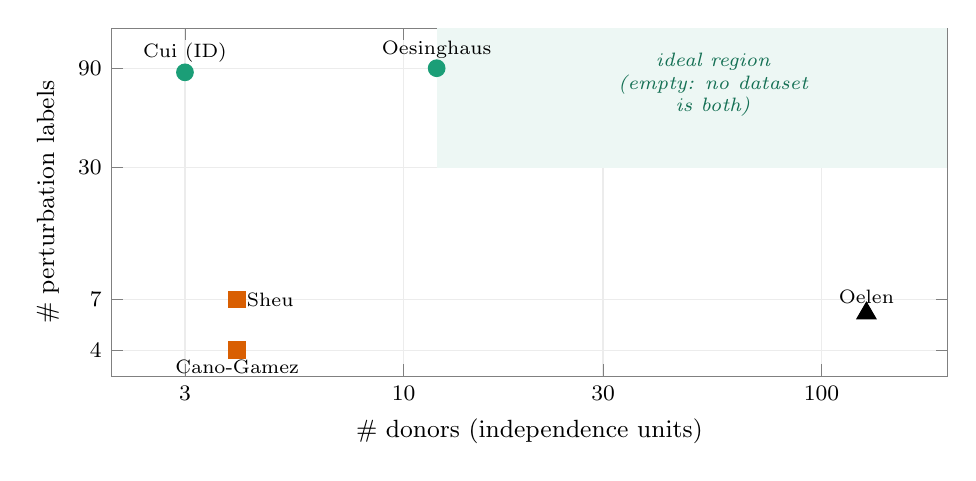
\begin{tikzpicture}
\begin{axis}[
  width=12.2cm, height=6.0cm,
  xmode=log, ymode=log, log basis x=10, log basis y=10,
  xlabel={\# donors (independence units)}, ylabel={\# perturbation labels},
  xmin=2, xmax=200, ymin=3, ymax=140,
  xtick={3,10,30,100}, xticklabels={3,10,30,100},
  ytick={4,7,30,90}, yticklabels={4,7,30,90},
  tick label style={font=\footnotesize}, label style={font=\small},
  axis line style={draw=gray}, grid=both, grid style={gray!15},
]
% "ideal" region: many donors AND many labels (currently empty)
\fill[good!8] (axis cs:12,30) rectangle (axis cs:200,140);
\node[good!70!black,font=\scriptsize\itshape,align=center] at (axis cs:55,75)
  {ideal region\\(empty: no dataset\\is both)};
% works (coupling + direction)
\addplot[only marks,mark=*,good,mark size=3pt] coordinates {(12,90) (3,86)};
% partial
\addplot[only marks,mark=square*,mid,mark size=3pt] coordinates {(4,7) (4,4)};
% scale milestone only
\addplot[only marks,mark=triangle*,scale,mark size=4pt] coordinates {(128,6)};
\node[anchor=south,font=\scriptsize] at (axis cs:12,90) {Oesinghaus};
\node[anchor=south,font=\scriptsize] at (axis cs:3,86) {Cui (ID)};
\node[anchor=west,font=\scriptsize] at (axis cs:4,7) {Sheu};
\node[anchor=north,font=\scriptsize] at (axis cs:4,4) {Cano-Gamez};
\node[anchor=south,font=\scriptsize] at (axis cs:128,6) {Oelen};
\end{axis}
\end{tikzpicture}
\caption*{\textbf{Figure 1.} The method needs \emph{both} many donors (powered null) \emph{and} many labels (stable degree correction). \textcolor{good}{Green}: coupling+direction work; \textcolor{mid}{orange}: partial; \textcolor{scale}{blue}: donor-scale milestone but too few labels. The joint ``ideal'' corner is empty---the standing gap.}
\end{figure}

\subsection{One line per dataset}
\begin{itemize}
\item \textbf{Oesinghaus} --- 90 cytokines on human PBMC; the method's home turf (enough labels \emph{and} donors). Best result: over-call halved to 31\% with rising recall; direction 88\%.
\item \textbf{Sheu} --- 7 TLR/cytokine stimuli on a \emph{500-gene targeted} mouse-BMDM panel. The narrow panel makes everything co-vary, so latent-geometry coupling fails (0/2); signature-space coupling rescues the textbook IFN cascades (2/2); direction 86\%.
\item \textbf{Cui / Immune Dictionary} --- 86 cytokines, mouse lymph node \emph{in vivo}. Whole-transcriptome with many labels $\Rightarrow$ clean coupling (88$\to$44\%, recall 6/7) and direction (83\%), even at only 3 donors (cell-level path).
\item \textbf{Cano-Gamez} --- 4 T-helper polarisation conditions on human CD4 T cells. Recovers the known Th17$\leftrightarrow$iTreg (TGF-$\beta$) coupling as \#1, but the 4 ``labels'' are parallel fates, not a cascade, so direction is undefined.
\item \textbf{Oelen} --- 3 pathogens$\times$2 time-points on human PBMC with \textbf{128 donors}. First time the donor-level null ran fully powered ($\sim$100 donors/pair). But 6 labels are too few for degree correction, and pathogens share one innate program, so the coupling benchmark is weak (1/3); the 3h$\to$24h progression direction is 2/3.
\end{itemize}

\subsection{Why they differ --- four metadata-driven rules}
\begin{enumerate}
\item \textbf{\# labels governs degree correction.} Works at $\gtrsim$15--20 conditions (Oes, Cui); \emph{fails} at 4--6 (Cano, Oelen)---too few nodes to estimate hub strength (over-call even rose on Oelen).
\item \textbf{\# donors governs the gate path.} $<$8 donors $\Rightarrow$ cell-level fallback (Sheu, Cui, Cano); $\geq$8 $\Rightarrow$ powered donor-level null; Oelen's 128 is the scale proof.
\item \textbf{Panel breadth governs the shared-activation confound.} A targeted 500-gene panel (Sheu) collapses latent geometry; signature space (specific genes) is panel-robust.
\item \textbf{Label semantics govern whether \emph{direction} exists.} Cytokine perturbations with known cascades $\Rightarrow$ direction (83--88\%); parallel fates (Cano) or pathogens (Oelen) give coupling/progression only, never cytokine$\to$cytokine direction.
\end{enumerate}
\textbf{Net.} The method needs \emph{many labels} (degree correction) $+$ \emph{$\geq$8 donors} (powered null) $+$ \emph{perturbation labels with directional relationships}. Oesinghaus uniquely has all three; every other dataset is missing one---exactly where it underperforms. The open need is a dataset that is simultaneously high-donor \emph{and} many-condition \emph{and} discriminative.

\section{Datasets without updated-method results (before this update)}
\textbf{COVID-19 (Stephenson/Haniffa) --- not a valid result yet.} We ran cross\_asym to recover disease-\emph{progression} direction (less-severe $=$ upstream) from $\sim$780K PBMCs over 5 severity grades (130 patients). The method's apparatus \emph{passed} its go/no-go gate (distinct-program ladder 100\%; monotone-intensity ladder 0\%, flagging the magnitude-confound regime). \textbf{But} the grade-vs-Healthy IG signatures were \emph{confounded} (cell-cycle genes, CITE-seq antibody tags, hemoglobin), so cross\_asym carried no severity signal (cross-accuracy 0.44 $<$ symmetric control 0.67; Kendall $\tau=-0.2$). The \textbf{coupling degree-fix and donor-level null were never applied here}. Treat as ``before this update''; a valid attempt requires cleaned signatures (drop ADT/hemoglobin/cell-cycle, grade-vs-grade contrasts) and the donor-level null.

\section*{Datasets \& references}
\begin{itemize}
\item Oesinghaus et al. (2024/25), \emph{A single-cell cytokine dictionary of human peripheral blood} --- 9.7M PBMC, 90 cytokines. \href{https://www.parsebiosciences.com/datasets/10-million-human-pbmcs-in-a-single-experiment/}{Parse 10M PBMC data}; \href{https://www.biorxiv.org/content/10.64898/2025.12.12.693897v1}{bioRxiv 2025.12.12.693897}.
\item Sheu et al.\ (2024), \emph{Molecular Cell} --- mouse BMDM, 500-gene panel. \href{https://www.ncbi.nlm.nih.gov/geo/query/acc.cgi?acc=GSE224518}{GEO GSE224518}.
\item Cui et al.\ (2024), \emph{Nature} 625:377 --- Immune Dictionary, 86 cytokines (mouse). \href{https://doi.org/10.1038/s41586-023-06816-9}{doi:10.1038/s41586-023-06816-9}; \href{https://singlecell.broadinstitute.org/single_cell/study/SCP2554}{SCP2554}.
\item Cano-Gamez et al.\ (2020), \emph{Nature Communications} 11:1801 --- CD4 T-cell cytokine responses. \href{https://doi.org/10.1038/s41467-020-15543-y}{doi:10.1038/s41467-020-15543-y}; \href{https://www.ebi.ac.uk/biostudies/studies/S-BSST2978}{BioStudies S-BSST2978}.
\item Oelen et al.\ (2022), \emph{Nature Communications} 13:3267 --- 1M-scBloodNL, 120-donor PBMC pathogen stimulation. \href{https://doi.org/10.1038/s41467-022-30893-5}{doi:10.1038/s41467-022-30893-5}; \href{https://eqtlgen.org/sc/datasets/1m-scbloodnl.html}{eQTLGen 1M-scBloodNL}.
\item Stephenson et al.\ (2021), \emph{Nature Medicine} 27:904 --- COVID-19 PBMC atlas, 130 patients. \href{https://doi.org/10.1038/s41591-021-01329-2}{doi:10.1038/s41591-021-01329-2}.
\end{itemize}

\end{document}
